\documentclass{beamer}
% \usetheme{default}
\usetheme{Boadilla}
\usepackage[utf8x]{inputenc}
\usepackage{default}
\usepackage{amsmath,amsthm,amsfonts,amssymb,graphicx,xcolor,ifthen}
\usepackage{algorithm,listings}
\usepackage{algorithmicx,algpseudocode}
\usepackage{multirow,array,lscape,chngpage,rotating}
\usepackage{colortbl,calc,fp}
\usepackage{setspace}

\usepackage{tikz}
\usetikzlibrary{snakes,patterns,shapes,calc}
\usepackage{pgfplots}
\pgfplotsset{width=7cm,compat=1.8}
\definecolor{darkgreen}{RGB}{0,127,0}

%%%%%%%%%%%%%%%%%%%%%%%%%%%%%%%%%%%%%%%%%%%%%%%%%%%%%%%%%%%%%%%%%%%%%%%%%%%%%%%

\newcommand{\smin}{s_\text{min}}
\newcommand{\smax}{s_\text{max}}
\newcommand{\qhi}{q_\text{hi}}
\newcommand{\qlo}{q_\text{lo}}
\newcommand{\zero}{\text{\textbf{0}}}
\newcommand{\Zproj}{Z^{\textit{proj}}}
\newcommand{\Zowa}{Z^{\textit{owa}}}
\newcommand{\nowa}{n^{\textit{owa}}}
\newcommand{\Q}{\mathcal{Q}}
\newcommand{\Y}{\mathcal{Y}}
\newcommand{\X}{\mathcal{X}}
\newcommand{\matW}{\hat W}
\newcommand{\matV}{\hat V}
\newcommand{\W}{{\mathcal{W}}}
\newcommand{\Wowa}{{\hat \W^{\textit{owa}}}}
\newcommand{\Waff}{\mathcal{\hat A}}
\newcommand{\WaffE}{{\mathcal{\hat A}_\E}}
\newcommand{\Wave}{{\mathcal{\hat W}^{ave}}}
\newcommand{\Wtave}{{\mathcal{W}^{ave,*}}}
\newcommand{\V}{\mathcal{V}}
\newcommand{\A}{\mathcal{A}}
\newcommand{\D}{\mathcal{D}}
\newcommand{\E}{\mathbb{E}}
\newcommand{\vv}{\mathbf{v}}
\newcommand{\z}{\mathbf{z}}
\newcommand{\x}{\mathbf{x}}
\newcommand{\y}{\mathbf{y}}
\newcommand{\w}{\mathbf{w}}
\newcommand{\wkl}{\hat\w^{kl}}
\newcommand{\ahat}{\hat\alpha}
\newcommand{\astar}{\alpha^*}
\newcommand{\afull}{\ahat^{\textit{full}}}
\newcommand{\wowa}{\hat\w^{owa}}
\newcommand{\wowafull}{\hat\w^{\textit{owa,full}}}
\newcommand{\wowastar}{\hat\w^{\textit{owa,*}}}
\newcommand{\wave}{\hat\w^{ave}}
\newcommand{\wtave}{\E\hat\w^{ave}}
\newcommand{\waver}{\hat\w^{ave,r}}
\newcommand{\wboot}{\hat\w^{boot}}
\newcommand{\wmle}{\hat\w^{erm}}
\newcommand{\wmlerr}{\hat\w^{erm,rr}}
\newcommand{\wmler}{\hat\w^{erm,r}}
\newcommand{\wstar}{{\w^{*}}}
\newcommand{\what}{{\hat\w}}
\newcommand{\wq}{\hat\w^{q}}
\newcommand{\wqstar}{\hat\w^{q^*}}
\newcommand{\reg}{r}
\newcommand{\loss}{\ell}
\newcommand{\Loss}{\mathcal{L}}
\newcommand{\R}{\mathbb{R}}

\newcommand{\trans}[1]{\ensuremath{{#1}^{\mathsf{T}}}}
\newcommand{\pinv}[1]{\ensuremath{{#1}^{\mathsf{\dagger}}}}
\newcommand{\ltwo}[1]{{\lVert {#1} \rVert}}
\newcommand{\ltwobig}[1]{{\left\lVert {#1} \right\rVert}}
\newcommand{\lone}[1]{{\lVert {#1} \rVert}_1}
\newcommand{\lzero}[1]{{\lVert {#1} \rVert}_0}
\newcommand{\proj}[1]{\pi_{{#1}}}
\newcommand{\prob}[1]{\Pr\left[{#1}\right]}

\newcommand{\I}{\mathcal I}
%\newcommand{\I^{-1}}{\I^{-1}}
\newcommand{\law}{\ensuremath{\xrightarrow{L}}}
\newcommand{\normal}[2]{\ensuremath{\mathcal{N}\left({{#1}},{{#2}}\right)}}

\DeclareMathOperator*{\argmin}{arg\,min}
\DeclareMathOperator*{\argmax}{arg\,max}
\DeclareMathOperator*{\vecspan}{span}
\DeclareMathOperator*{\affspan}{aff}
\DeclareMathOperator*{\subG}{subG}
\DeclareMathOperator*{\tr}{tr}

\definecolor{wmle}{RGB}{0,0,0}
%\definecolor{wmlei}{RGB}{230,159,0}
\definecolor{wmlei}{RGB}{150,100,0}
\definecolor{wave}{RGB}{40,090,233}
\definecolor{wboot}{RGB}{204,021,167}
\definecolor{wowa}{RGB}{0,158,115}

\definecolor{lightred}{RGB}{255,200,200}
\definecolor{lightgreen}{RGB}{200,255,200}
\definecolor{lightblue}{RGB}{200,200,255}
\definecolor{darkred}{RGB}{127,0,0}
\definecolor{darkgreen}{RGB}{0,127,0}
\definecolor{darkblue}{RGB}{0,0,127}
\definecolor{darkbrown}{RGB}{101,67,33}

\newcommand{\spacer}[1]{
    \begin{frame}
    \begin{center}
    \Huge\em{#1}
    \end{center}
    \end{frame}
}

\newcommand{\ignore}[1]{}

%%%%%%%%%%%%%%%%%%%%%%%%%%%%%%%%%%%%%%%%%%%%%%%%%%%%%%%%%%%%%%%%%%%%%%%%%%%%%%%

\author {Mike Izbicki}
\institute{UC Riverside}
\title[Dissertation Defense]{}
\date{August 23, 2017}

\begin{document}

\beamertemplatenavigationsymbolsempty

%%%%%%%%%%%%%%%%%%%%%%%%%%%%%%%%%%%%%%%%%%%%%%%%%%%%%%%%%%%%%%%%%%%%%%%%%%%%%%%


%\begin{frame}{}

%\begin{center}
%Dissertation Proposal
%\end{center}
%
%\vspace{0.25in}

\begin{center}
\LARGE
Divide and Conquer Algorithms 

for Faster Machine Learning
\end{center}
\begin{center}
Mike Izbicki
\end{center}

\vspace{0.05in}
%\begin{center}
%by Mike Izbicki
%\end{center}

\begin{center}
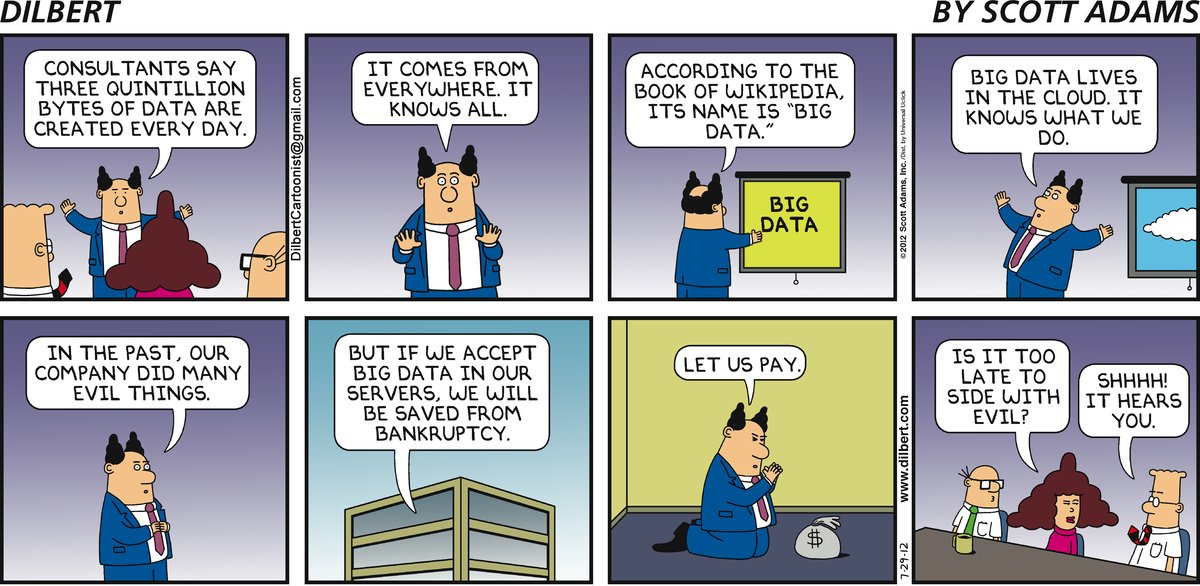
\includegraphics[width=0.985\textwidth]{img-presentation/dilbert}
\end{center}
\end{frame}

%%%%%%%%%%%%%%%%%%%%%%%%%%%%%%%%%%%%%%%%%%%%%%%%%%%%%%%%%%%%%%%%%%%%%%%%%%%%%%%%

\ignore{
\begin{frame}{}

\begin{center}
Dissertation Defense
\end{center}

\vspace{0.25in}

\begin{center}
\Huge
Divide and Conquer Algorithms 

for Faster Machine Learning
\end{center}

\vspace{0.25in}
\begin{center}
by Mike Izbicki
\end{center}
\end{frame}
}

%\begin{frame}{Why faster machine learning?}

\vspace{0.05in}
\begin{tikzpicture}

%%%%%%%%%%%%%%%%%%%%%%%%%%%%%%%%%%%%%%%%

\node[text width=10cm] at (0,0) {
Facebook generates more than 200 terabytes of data per day (Facebook blog, 2014)
};

%\uncover<1>{
%\foreach \i in {1,...,20}
%\foreach \j in {1,...,10}
%{
    %\node at (0.5*\i-4.25,-2-0.5*\j) {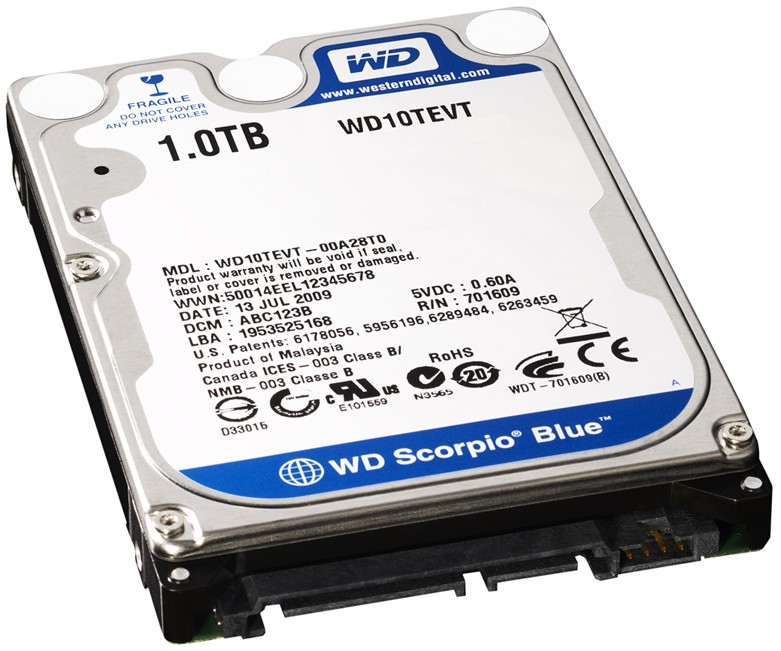
\includegraphics[width=0.4cm]{img-presentation/1tb}};
%}
%\node at (-4,-2) {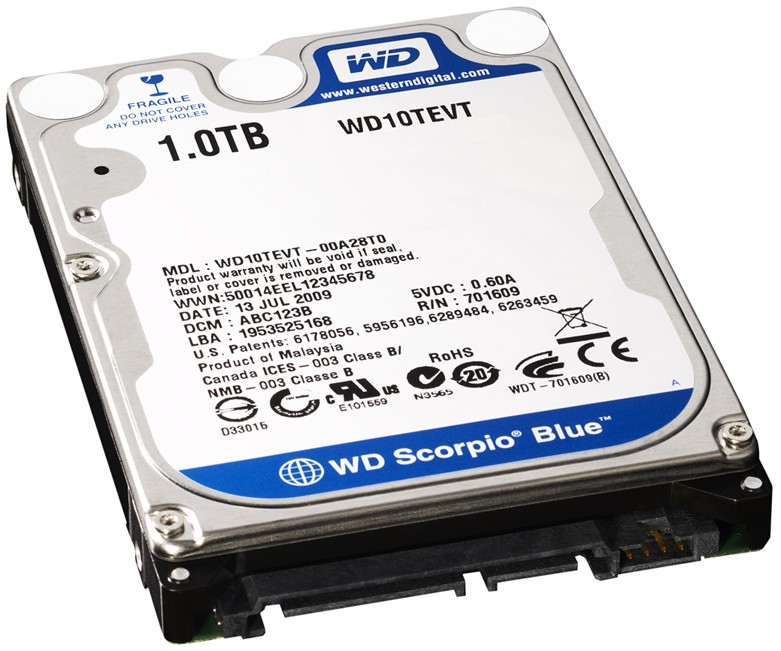
\includegraphics[width=3cm]{img-presentation/1tb}};
%}

%%%%%%%%%%%%%%%%%%%%%%%%%%%%%%%%%%%%%%%%

\uncover<2-9> {
\node at (-4.35,-0.9) {
\includegraphics[width=0.2cm]{img-presentation/dot}};
\node[text width=10cm] at (1,-0.9) {
    includes uploaded images%
    {\uncover<4-9>{, messages}}%
    {\uncover<5-9>{, and user likes}}
};
\uncover<2-6>{\node at (-2,-3.5) {
    %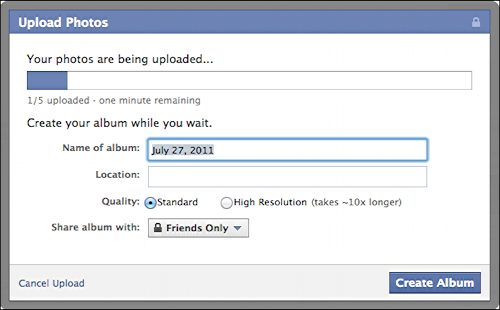
\includegraphics[width=5cm]{img-presentation/facebook-upload-photo-computer-6}
    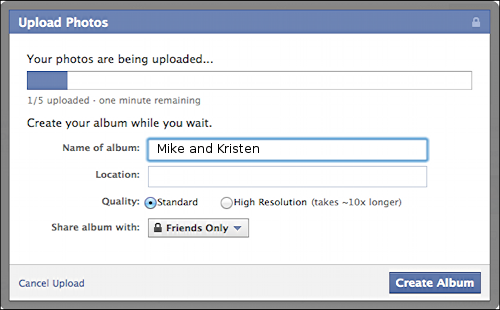
\includegraphics[width=5cm]{img-presentation/fb-upload}
};}
\uncover<2-6>{\node at (1.75,-3.75) {
    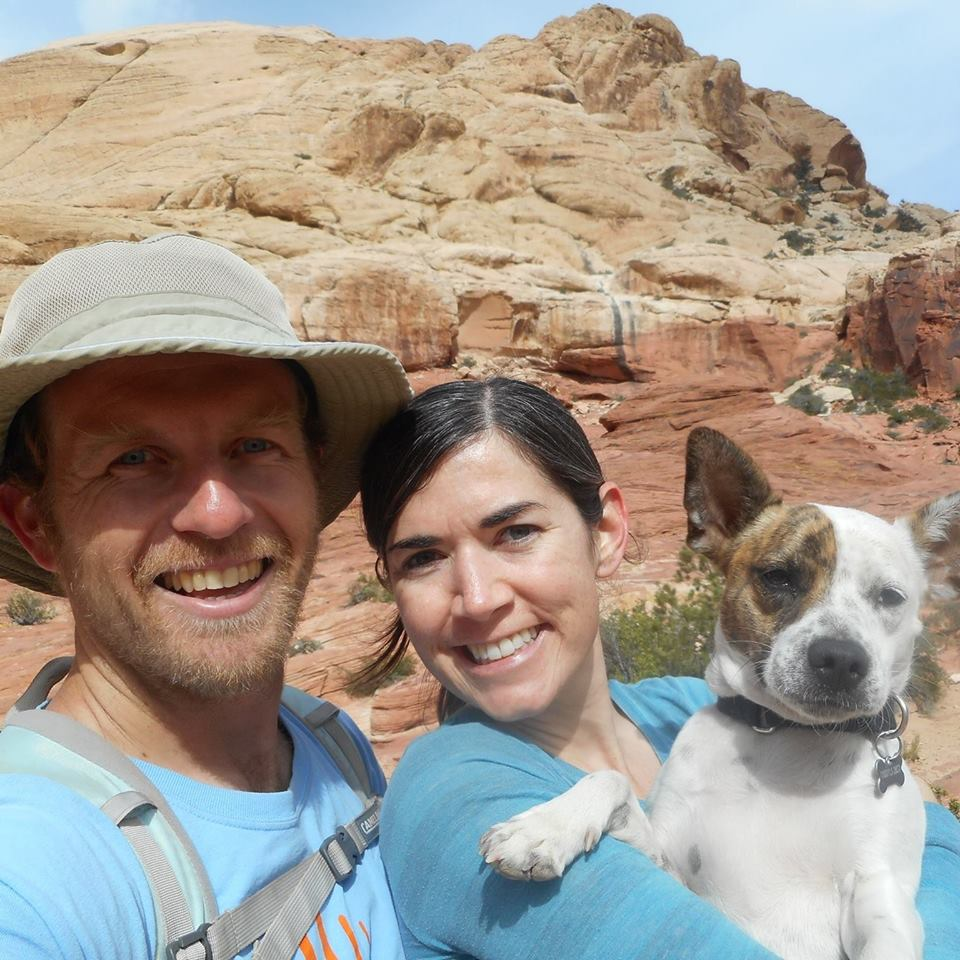
\includegraphics[width=3cm]{img-presentation/dog}
};}
\uncover<4-6>{\node at (5,-4.25) {
    %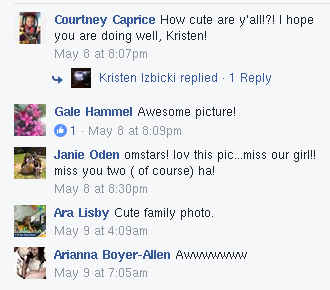
\includegraphics[width=3cm]{img-presentation/dog-message}
    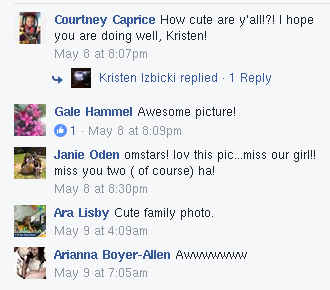
\includegraphics[width=4cm]{img-presentation/dog-message}
};}
\uncover<5-6>{\node at (3.5,-6.5) {
    
\includegraphics[width=3cm]{img-presentation/fb-like}
};}
}

%%%%%%%%%%%%%%%%%%%%%%%%%%%%%%%%%%%%%%%%

\uncover<6-9>{
\node at (-4.35,-1.5) {
\includegraphics[width=0.2cm]{img-presentation/dot}};
\node[text width=10cm] at (1,-1.5) {
    machine learning algorithms use this data to solve problems
};
\uncover<7-9>{
\node[text width=10cm] at (1,-2.0) {like identifying people in images
{\uncover<8-9>{and displaying profitable ads}}};
}

\uncover<7-8>{
\node at (-2,-5) {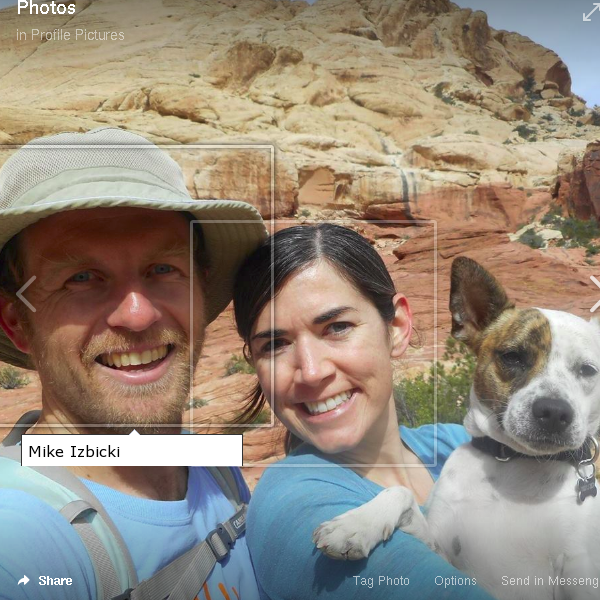
\includegraphics[width=5cm] {img-presentation/fb-faces2}};
}
\uncover<8>{\node at (4,-5) {
    
\includegraphics[width=5cm] {img-presentation/fb-ad-hiking}
};}
}

%%%%%%%%%%%%%%%%%%%%%%%%%%%%%%%%%%%%%%%%

\uncover<9> {
\node[text width=12cm] at (1,-2.6) {\textbf{Challenge:} we need new, faster algorithms to process this data};
%\node[text width=6cm] at (-2,-3.1) {Facebook has ``an estimated hundreds of thousands'' of computers};
%\node at (4,-5) {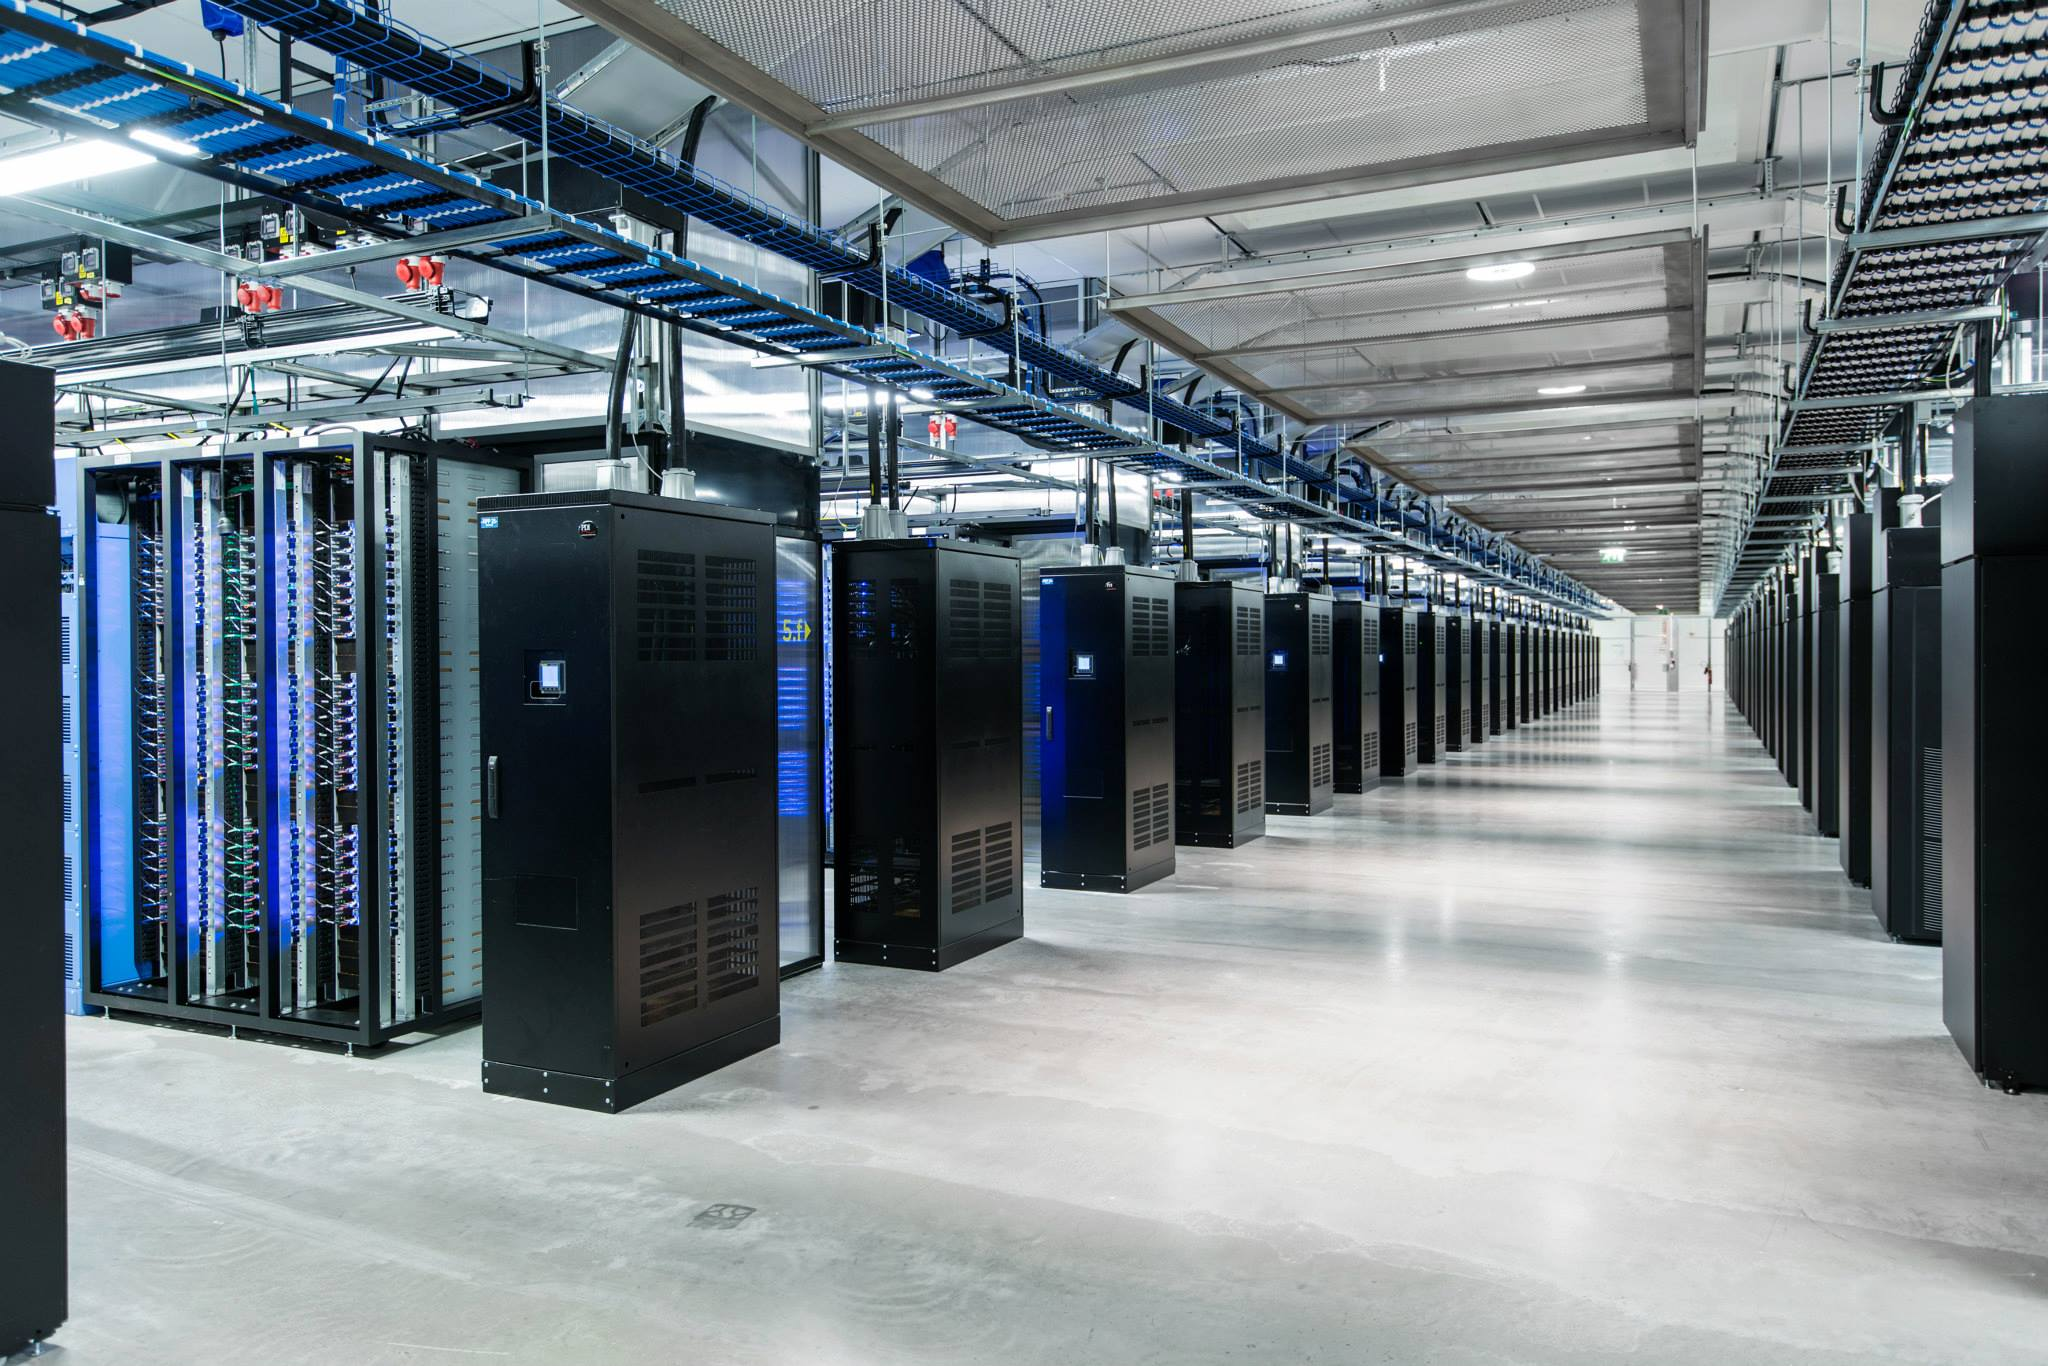
\includegraphics[width=6cm]{img-presentation/facebook_10969}};
}

%%%%%%%%%%%%%%%%%%%%%%%%%%%%%%%%%%%%%%%%

\end{tikzpicture}

%This data is stored on ``hundreds of thousands'' of computers
%
%(Facebook Datacenter FAQ)

\end{frame}

%%%%%%%%%%%%%%%%%%%%%%%%%%%%%%%%%%%%%%%%%%%%%%%%%%%%%%%%%%%%%%%%%%%%%%%%%%%%%%%%

\begin{frame}{Many organizations need faster machine learning}

\begin{itemize}
\item 
computer companies

\vspace{0.05in}
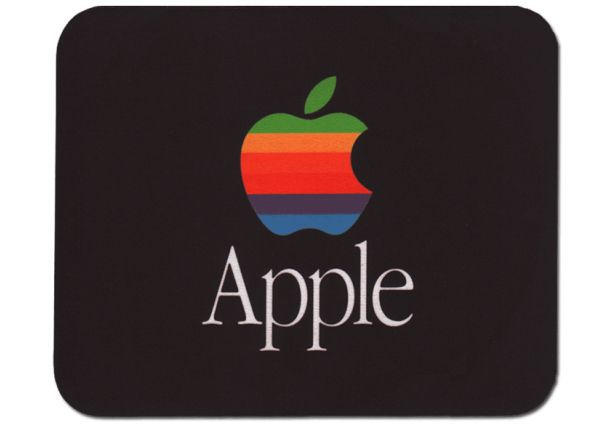
\includegraphics[height=1cm]{img-presentation/apple}~~~

\includegraphics[height=1cm]{img-presentation/ms}~~~

\includegraphics[height=1cm]{img-presentation/google}

\vspace{0.05in}

\includegraphics[height=1cm]{img-presentation/linkedin}~~~

\includegraphics[height=1cm]{img-presentation/yahoo}

\pause
\vspace{0.1in}
\item
traditional engineering

\vspace{0.05in}

\includegraphics[height=1cm]{img-presentation/pfizer}~~~

\includegraphics[height=1cm]{img-presentation/gm}

\pause
\vspace{0.1in}
\item 
pure scientific research

\vspace{0.05in}

\includegraphics[height=1cm]{img-presentation/nasa}~~~
%
\includegraphics[height=1cm]{img-presentation/nsf}~~~

\includegraphics[height=1cm]{img-presentation/cern}~~~

\includegraphics[height=1cm]{img-presentation/nih}

\end{itemize}

\end{frame}

%%%%%%%%%%%%%%%%%%%%%%%%%%%%%%%%%%%%%%%%%%%%%%%%%%%%%%%%%%%%%%%%%%%%%%%%%%%%%%%%

\begin{frame}{My research}
\textbf{Goal:} 
%Goal:
%\begin{itemize}
%\item
generic techniques that make machine learning faster for everyone

%for all these organizations
%\end{itemize}

\pause
\vspace{0.15in}
Examples
\begin{itemize}
\item
ad-click data from the Tencent search engine

(improve ad revenue for a given computational budget)

\vspace{-1.5cm}
\begin{tikzpicture}
\node at (0,0) {};
\node at (10,0) {
\includegraphics[width=2cm]{img-presentation/tencent}};
\end{tikzpicture}
%\vspace{-1cm}

\pause
\item
protein data bank

(first analysis of approximately 100,000 human 

proteins using random walk graph kernels)

\vspace{-1.5cm}
\begin{tikzpicture}
\node at (0,0) {};
\node at (9.5,0) {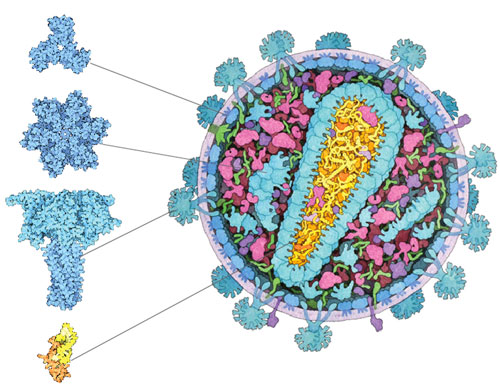
\includegraphics[width=2.5cm]{img-presentation/pdb}};
\end{tikzpicture}

\pause
\vspace{-0.4cm}
\item
Flickr creative commons images

(find patterns in 1.5 million images on a single machine)
\end{itemize}

\vspace{-0.8cm}
\begin{tikzpicture}
\node at (0,0) {};
\node at (11,0) {
\includegraphics[width=1.3cm]{img-presentation/flikr}};
\end{tikzpicture}

\pause
\vspace{-0.15in}
Main contributions are \textbf{theoretical} and \textbf{more general}
\end{frame}

%\newcommand{\new}{(new)}

\begin{frame}{Outline of my contributions}

Mergeable learning algorithms
\begin{itemize}
    %\item simple example
    \item popular class of distributed learning algorithms
    \item fast cross validation algorithm
\end{itemize}

\vspace{0.1in}
Optimal weighted average (OWA) merge procedure
\begin{itemize}
    \item better theoretical guarantees than previous methods
    \item experiments on large scale ad-click data
\end{itemize}

\vspace{0.1in}
Cover tree data structure for nearest neighbor queries
\begin{itemize}
    \item merge procedure
    \item improved analysis of runtimes
    \item new notion of metric dimension 
    \item experiments on large scale protein and image data
\end{itemize}


%\vspace{-2in}
%\begin{tikzpicture}
%\node at (0,0) {};
%\node at (10,0) {
\includegraphics[width=2cm]{img-presentation/tencent}};
%\node at (9.5,-2.5) {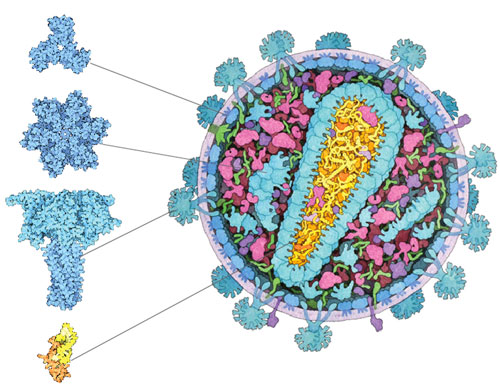
\includegraphics[width=2.5cm]{img-presentation/pdb}};
%\node at (11,-4) {
\includegraphics[width=1.3cm]{img-presentation/flikr}};
%\end{tikzpicture}

\end{frame}


%
%\spacer{mergeable learning algorithms}
%\tikzstyle{blackbox}=[shape=rectangle, draw, fill=black, draw=white, draw opacity=0, line width=0.15in, text=white, minimum size=0.3in]
\tikzstyle{whitebox}=[shape=rectangle, draw, fill=white, draw=black, minimum size=0.3in]

%%%%%%%%%%%%%%%%%%%%%%%%%%%%%%%%%%%%%%%%

\begin{frame}{Mergeable learning algorithms use 1 round of MapReduce}
\centering
\begin{tikzpicture}[line width=2pt]
\node[color=white] at (-6,-1) {\begin{sideways} partition \end{sideways}};
\node[minimum width=12cm,minimum height=1.7cm,fill=white,opacity=0.1] at (-0.5,-1) {};

\node (long) {\includegraphics[width=4in]{/home/user/docs/research/presentation_lib/dna/long}};

\uncover<1> {
\node at (-3,-1) {big data};
%\node at (-0.5,-3) {\rotatebox{90}{training}};
\node at (-1.1,-3) {{training}};
\node at (1.2,-5.8) {model};
}

\node[blackbox] (mc) [below of = long, node distance = 2.3in] {};

\draw[->,line width=2pt] (long) to (mc);


%%%%%%%%%%%%%%%%%%%%%%%%%%%%%%%%%%%%%%%
\pause
\node[minimum width=5in,minimum height=2.5in,fill=white] at (0,-1.05in) {};

\node at (-6,-1) {\begin{sideways} partition \end{sideways}};
\node[minimum width=12cm,minimum height=1.7cm,fill=green,opacity=0.1] at (-0.5,-1) {};

\node at (-6,-3) {\begin{sideways} map \end{sideways}};
\node[minimum width=12cm,minimum height=1.7cm,fill=green,opacity=0.1] at (-0.5,-3) {};

\node at (-6,-5) {\begin{sideways} reduce \end{sideways}};
\node[minimum width=12cm,minimum height=1.7cm,fill=green,opacity=0.1] at (-0.5,-5) {};

\node (long) {\includegraphics[width=4in]{/home/user/docs/research/presentation_lib/dna/long}};

\node (short1) at (-1.5in,-0.75in) {\includegraphics[width=1in]{/home/user/docs/research/presentation_lib/dna/short3}};
\node (short2) at (-0.5in,-0.75in) {\includegraphics[width=1in]{/home/user/docs/research/presentation_lib/dna/short2}};
\node (short3) at (0.5in,-0.75in) {\includegraphics[width=1in]{/home/user/docs/research/presentation_lib/dna/short1}};
\node (short4) at (1.5in,-0.75in) {\includegraphics[width=1in]{/home/user/docs/research/presentation_lib/dna/short2}};

\node[blackbox] (mc1) [below of=short1, node distance = 0.8in] {};
\node[blackbox] (mc2) [below of=short2, node distance = 0.8in] {};
\node[blackbox] (mc3) [below of=short3, node distance = 0.8in] {};
\node[blackbox] (mc4) [below of=short4, node distance = 0.8in] {};

\node[blackbox] at (-1.0125in,-2in) [out=270 ,in=180] (mc12) {};
\node[blackbox] at (1.0125in,-2in) (mc34) {};

\node[blackbox] (mc) [below of = long, node distance = 2.3in] {};

\draw[->] (-1.5in,-0.25in) to (-1.5in,-0.4in);
\draw[->] (-0.5in,-0.25in) to (-0.5in,-0.4in);
\draw[->] (0.5in,-0.25in) to (0.5in,-0.4in);
\draw[->] (1.5in,-0.25in) to (1.5in,-0.4in);
%\draw[->] (long) to (short1);
%\draw[->] (long) to (short2);
%\draw[->] (long) to (short3);

\draw[->] (short1) to (mc1);
\draw[->] (short2) to (mc2);
\draw[->] (short3) to (mc3);
\draw[->] (short4) to (mc4);

\draw[->] (mc1.south) to (mc12);
\draw[->] (mc2.south) to (mc12);
\draw[->] (mc3.south) to (mc34);
\draw[->] (mc4.south) to (mc34);

\draw[->] (mc12) to (mc);
\draw[->] (mc34) to (mc);

%\uncover<3>{
%\node[draw=red, line width = 2pt, fill=white, minimum width=4in, minimum height=1.5in] at (-0.1in,-0.4in) {
    %\parbox{3.5in}{
    %Computations over finite, constant-time monoids are complete in the parallel complexity class $\mathbb{NC}^1$.
%
    %$$
    %\mathbb{NC}^1 \subseteq \mathbb{NC} \subseteq \mathbb{P} \subseteq \mathbb{NP}
    %$$
    %}
%};}

\uncover<3> {
\node at (-0.5,-6.75) {\color{darkgreen} \textbf{
    Advantages: fast, implement with standard libraries, privacy 
}};
}

\uncover<4-5>{
\draw[color=red,line width=2pt,fill=lightred, opacity=0.5] (-2.55,-4.3) ellipse (2cm and 1.3cm);
\draw[color=red,line width=2pt                           ] (-2.55,-4.3) ellipse (2cm and 1.3cm);

\node at (-3.3,-6.3) {\color{red} \textbf{
    How do we merge two models?
    }};
}

\uncover<5> {
\node at (-3.1,-6.9) {\color{red} \textbf{What else does merging give us?}};
}

\onslide<1->
\end{tikzpicture}
\end{frame}


%%%%%%%%%%%%%%%%%%%%%%%%%%%%%%%%%%%%%%%%%%%%%%%%%%%%%%%%%%%%%%%%%%%%%%%%%%%%%%%


%\begin{frame}{Mergeable estimators are popular}
    \vspace{0.4in}
    \uncover<2>{
    
\begin{tikzpicture}
        \draw[draw=white,opacity=0.75,fill=yellow] (0,0) -- (12.25,0) -- (12.25,1.55) -- (0,1.55);
    \end{tikzpicture}
}
    \vspace{-1.275in}

    \setstretch{0.8}{
\begin{itemize}
    \item
    methods with closed form solution
    %(\textbf 3 solutions)

    {\tiny linear exponential families, naive bayes, ridge regression}

    \vspace{0.1in}
    \item 
    regularized loss minimization
    %(\textbf 9 solutions)

    {\tiny (Mergu and Ghosh, 2003; McDonald et al., 2009; Zinkevich et al., 2010; Zhang et al., 2012, 2013b; Liu and Ihler, 2014; Battey et al., 2015; Han and Liu, 2016; Lee et al., 2017)}

    \vspace{0.1in}
    \item 
    principle component analysis
    %(\textbf 2 solutions)

    {\tiny (Qu et al., 2001; Liang et al., 2013)}

    \vspace{0.1in}
    \item 
    submodular optimization
    %(\textbf 6 solutions)
    
    {\tiny (Mirzasoleiman et al., 2013; Barbosa et al., 2015; Malkomes et al., 2015; Bhaskara et al., 2016; Barbosa et al., 2016; Mirzasoleiman et al., 2016)}

    \vspace{0.1in}
    \item 
    variational inference
    %(\textbf 3 solutions)

    {\tiny (Broderick et al., 2013; Campbell and How, 2014; Neiswanger et al., 2015)}

    \vspace{0.1in}
    \item 
    markov chain monte carlo
    %(\textbf 8 solutions)
    
    {\tiny (Wang and Dunson, 2013; Minsker et al., 2014; Neiswanger et al., 2014; Wang et al., 2015; White et al., 2015; Srivastava et al., 2015; Nemeth and Sherlock, 2016; Scott et al., 2016)}
\end{itemize}
}
\end{frame}

%\begin{frame}{The regularized loss minimization (RLM) framework}

Solve the following optimization
\begin{equation}
\wmle = \argmin_{\w\in\W} \sum_{(y,\x)\in Z} \loss(y;\trans\w\x) + \lambda\reg(\w)
\end{equation}
where
\begin{itemize}
\item $Z$ is a dataset with $mn$ points ($m$ machines each with $n$ points)
\item $y\in\Y\subset\mathbb R$
\item $\x\in\X\subset\mathbb R^d$
\item $\w\in\W\subset\mathbb R^d$
\item $\loss$ is the (not necessarily convex) loss function
\item $\reg : \W\to\mathbb R$ is the regularization function
\end{itemize}

\vspace{0.15in}
\textbf{Theory:} the statistical error decays as $\ltwo{\wstar-\wmle} \le O(\sqrt{d/mn})$ where $\wstar$ is the optimal parameter in $\W$.
\end{frame}

%%%%%%%%%%%%%%%%%%%%%%%%%%%%%%%%%%%%%%%%

\begin{frame}{RLM for ridge regression can be exactly parallelized}
In ridge regression, we set
\begin{equation}
\loss(\y,\trans\w\x) = \ltwo{\y-\trans\w\x}^2 
~~~ \text{and} ~~~
\reg(\w) = \ltwo{\w}^2,
\end{equation}
so the estimator has closed form solution
\begin{equation}
\wmlerr = (\trans X X - \lambda I)^{-1}(\trans X Y),
\end{equation}
where $X : \R^{mn\times d}$ and $Y : \R^{mn\times 1}$ are the design and response matrices.

\pause
\hrulefill
\vspace{0.1in}

In the \textbf{map} phase, each machine $i$ calculates
\begin{equation}
A_i = \trans X_i X_i
~~~\text{and}~~~
B_i = \trans X_i Y_i
\end{equation}
where $X_i : \R^{n\times d}$ and $Y : \R^{n\times 1}$ are the design and response matrices for only the data on machine $i$.
In the \textbf{reduce} phase, calculate
\begin{equation}
\textstyle
\wmlerr = \left(\sum_{i=1}^m A_i - \lambda I\right)^{-1}\left(\sum_{i=1}^m B_i\right).
\end{equation}
\end{frame}

%\begin{frame}{The averaging distributed estimator}

Procedure:

\begin{itemize}

%\item Assign to each machine $i\in\{1...m\}$ a dataset $Z_i$ with $n$ datapoints

\item In the \textbf{map} phase, each machine calculates the local ERM

\begin{equation}
\wmle_i = \argmin_{\w} \sum_{(y,\x)\in Z_i} \loss(y;\trans\w\x) + \lambda\reg(\w)
\end{equation}

where $Z_i$ is the local data set of machine $i$.

%\item A central server calculates the averaging estimator

\item
In the \textbf{reduce} phase, we calculate
\begin{equation}
\wave = \frac{1}{m}\sum_{i=1}^m \wmle_i
.
\end{equation}

\end{itemize}

\textbf{Theory:}

\vspace{-0.2in}
\begin{equation}
\ltwo{\wstar-\wave} \le 
\ltwo{\wstar-\E\wave} 
+
\ltwo{\E\wave-\wave} 
\end{equation}

\hspace{1.9in}
$O(\sqrt{d/n})$
\hspace{0.3in}
$O(\sqrt{d/mn})$

\vspace{0.15in}
(McDonald et al., 2009; Zhang et al., 2012; Rosenblatt and Nadler, 2016)
\end{frame}

%%%%%%%%%%%%%%%%%%%%%%%%%%%%%%%%%%%%%%%%

\begin{frame}{Can we do better than averaging? Yes!}

Estimators with bias reduction
\begin{itemize}
%\item
%If the datasets on each machine overlap each other, then there is a reduction in bias
%(Zinkevich et al., 2012)
%
%\textcolor{darkgreen}{Good: simple}
%; 
%\textcolor{red}{Bad: different problem setup}

\item
Estimate the bias via a bootstrap subsample (Zhang et al., 2012)

\textcolor{darkgreen}{easy to implement}
; 
\textcolor{red}{suboptimal scalability}

\item
Closed form formula for the optimal $\lambda$ in kernel ridge regeression (Zhang et al., 2013)

\textcolor{darkgreen}{easy to implement}
; 
\textcolor{red}{applies to limited models}

\item
Closed form estimates of the bias in certain L1 penalized models

(Lee et al., 2015; Battey et al., 2015)

\textcolor{darkgreen}{easy to implement}
; 
\textcolor{red}{applies to limited models}

\item
Averaging the models with the KL average (Liu and Ihler, 2014)

\textcolor{darkgreen}{good statistical guarantees}
; 
\textcolor{red}{must solve intractable integral}

\end{itemize}

\pause

Goal: 
\begin{itemize}
    \item easy to implement 
    \item good statistical guarantees 
    \item efficiently calculatable
\end{itemize}

%\vspace{0.15in}
%Impossibility theorems
%
%\begin{itemize}

%\item
%At least $\Omega(m\min\{n,d\})$ bits must be transferred for $O(\sqrt{d/mn})$ error rate
%(Braverman et al., 2016)

%\item
%No merged estimator can achieve $O(\sqrt{d/mn})$ error rate
%
%(Zhang et al. 2013; Shamir 2014; Garg et al. 2014; Liu and Ihler 2014)\!\!\!\!
%
%%\begin{itemize}
%\item
%All results assume that the merge procedure does not depend on data
%%\end{itemize}
%
%\end{itemize}

\end{frame}



%
%\spacer{the optimal weighted average}
%%%%%%%%%%%%%%%%%%%%%%%%%%%%%%%%%%%%%%%%%

\begin{frame}
\frametitle{The \uncover<1-6>{full} optimal weighted average (OWA)}

Procedure:
\uncover<2-7>{
\vspace{0.1in}
\begin{itemize}
\item
In the \textbf{map} phase,
calculate the $\wmle_i$ as before
}

\uncover<3-7>{
\vspace{0.1in}
\item
In the \textbf{reduce} phase,
%On the second round, 
\begin{itemize}
\item 
Let $\Wowa = \vecspan\{\wmle_i\}_{i=1}^m$\uncover<7>{, $Z^{owa}$ be a new dataset}
}

\uncover<4-7>{
\item Calculate
\begin{align}
\label{eq:afull}
\wowa{}^{\uncover<1-6>{,full}} &= \argmin_{\w\in\Wowa} \sum _{(\x,y)\in Z^{\textit{\uncover<7>{owa}}}} \loss\left(y,\trans\x\w \right)
+
\lambda \reg(\w)
\end{align}
}
\end{itemize}
\end{itemize} 

%\vspace{0.1in}
Graphical Intuition
\begin{center}
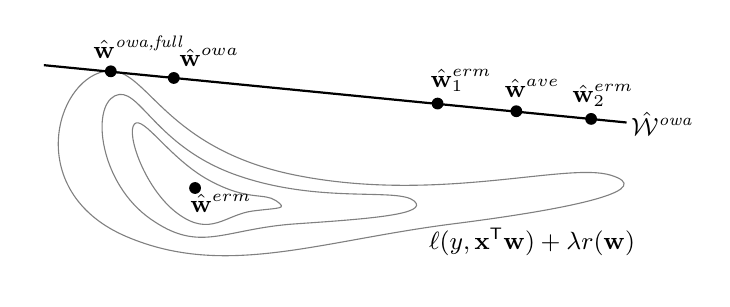
\begin{tikzpicture}
    [
    dot/.style = {minimum width=0.15cm,inner sep=0pt,line width=0pt,fill,circle,black,font=\small}
    , yscale=0.65
    ]
\small
\draw[gray] plot [smooth cycle,tension=1] coordinates {(-0.5,-0.75) (-1.05,1) (-0.1,-0.1) (0.75,-0.5) (0.45,-0.7) };
\draw[gray] plot [smooth cycle,tension=1] coordinates {(-0.85,-0.85) (-1.3,1.55) (0.25,0) (2.5,-0.5) (1,-0.95)};
\draw[gray] plot [smooth cycle,tension=1] coordinates {(-1.15,-1.2) (-1.5,2) (1,0) (5,0) (3,-0.95)};

\node[dot] (wstar) at (-0.28,-0.25) {};
\node at (0.05,-0.55) {$\wmle$};

\uncover<3-7>{
\draw[thick] (-2.2,2.15) -- (5.2,1.03);
\node at (5.65,1.0) {$\Wowa$};
}

\uncover<2-7>{
%\node[dot] (wstarproj) at (0.1,1.8) {};
%\draw (wstar) -- (wstarproj);
%\draw (0.07,1.65) -- (0.23,1.62) -- (0.26,1.78);

%\node[dot] (wavestar) at (4,0.5) {};
%\node                 at (4.5,0.3) {$\E\wave$};
\node[dot] (wave) at (2.80,1.40) {};
\node at (3.1,1.85) {$\wmle_1$};
\node[dot] (wave) at (4.75,1.10) {};
\node at (4.9,1.55) {$\wmle_2$};
%\node[dot] (wave) at (3.8,1.25) {};

}

\uncover<4-7>{
\node[dot] at (-1.35,2.03) {};
\node at (-1.0,2.5) {$\wowafull$};
}

\uncover<6-7>{
\node[dot] (wave) at (3.8,1.25) {};
\node at (4.0,1.7) {$\wave$};
}

\uncover<7>{
\node[dot] at (-0.55,1.9) {};
\node at (-0.1,2.3) {$\wowa$};
}

\node at (4,-1.3) {$\loss(y,\trans\x\w)+\lambda \reg(\w)$};
%\node at (6.95,1.0) {$\Wowa = \vecspan\{\wmle_i\}_{i=1}^m$};

\end{tikzpicture}
\end{center}

\end{frame}

%%%%%%%%%%%%%%%%%%%%%%%%%%%%%%%%%%%%%%%%

\begin{frame}{Efficiently calculating $\wowa$}

%Let $\matW = \bigg(\wmle_1, \wmle_2, ..., \wmle_m\bigg) \in \mathbb R^{d\times m}$
%
%\vspace{0.1in}
%Then every $\w\in\Wowa$ can be written as $\w=\matW\alpha$, where $\alpha\in\mathbb R^m$

\vspace{0.1in}
We can rewrite $\wowa$ as
%$\wowa = \matW \ahat$
%where
\begin{align}
\wowa &= \matW \ahat
\\
\label{eq:afull}
\ahat &= \argmax_{\alpha\in\mathbb R^m} \sum _{(\x,y)\in \Zowa} \loss\left(y,\trans\x \matW \alpha \right)
+
\lambda \reg(\matW\alpha)
\\
\matW &= \bigg(\wmle_1, \wmle_2, ..., \wmle_m\bigg) \in \mathbb R^{d\times m}
\end{align}

%In the second round of communication
%\begin{itemize}
%\item Each machine transmits $\trans\x\matW$ for each data point in $\Zowa$
%\item This is $O(m)$ bits per data point 
%
%~~~~~~~~~$O(m\nowa)$ bits per machine
%
%~~~~~~~~~$O(m^2\nowa)$ bits total
%%\item Whenever $m\nowa < d$, fewer bits are transfered than the first round
%\end{itemize}

\pause
Notice that:
\begin{itemize}
%\item
%The merging procedure depends on the data,
%so existing impossibility theorems do not apply.

%\pause
\item
The $\ahat$ optimization happens in a low dimensional subspace, so few datapoints are needed.

\pause
\item
The $\trans\x\matW$ in $(11)$ does not depend on $\alpha$, so needs to be computed only once (instead of each iteration).

%\pause
%\item
%The $\Zowa$ dataset should be stored already on the reduce server.
%
%(In the paper, we provide an algorithm for efficiently communicating the $\Zowa$ dataset to the reducer if needed.)

\end{itemize}

\end{frame}



\newtheorem*{sgt}{The subgaussian tail condition}
\newtheorem*{thm1}{Theorem 1: error of $\wowafull$}
\newtheorem*{thm2}{Theorem 2: error of $\wowa$}

\pgfmathdeclarefunction{gauss}{2}{%
  \pgfmathparse{1/(#2*sqrt(2*pi))*exp(-((x-#1)^2)/(2*#2^2))}%
}

\pgfmathdeclarefunction{multi}{2}{%
    \pgfmathparse{(0.0001+abs(sin((x-0.2)/100)))*1/(#2*sqrt(2*pi))*exp(-((x-0.4)^2)/(2*#2^2))}%
}

\pgfmathdeclarefunction{truncated}{2}{%
    \pgfmathparse{(abs(x)<1.5)*1/(#2*sqrt(2*pi))*exp(-((x-#1)^2)/(2*#2^2))}%
}

\newcommand{\mkdensity}[2]{
\begin{axis}[
  no markers, 
  domain=-3.5:3.5, 
  samples=100,
  axis lines=left, 
  xlabel=$\ltwo{\wstar-\wmle_i}$,
  every axis y label/.style={at=(current axis.above origin),anchor=south},
  every axis x label/.style={at=(current axis.right of origin),anchor=west},
  height=4.5cm, 
  width=10cm,
  xtick=0, 
  ytick=\empty,
  enlargelimits=false, 
  clip=false, 
  axis on top,
  grid = major
  ]
%\addplot [very thick,cyan!50!black] {gauss(0, 1)};
  \addplot [very thick,cyan!50!black] {{#2}};
\end{axis}
\node[text width=10cm] at (4,3.5) {Example: {#1}};
\node at (-0.5,1.5) {\rotatebox{90}{density}};
}

\begin{frame}{OWA's theoretical analysis}

%%%%%%%%%%%%%%%%%%%%%%%%%%%%%%%%%%%%%%%%

\begin{sgt}
%Let $\wmle_i$ be a linear estimator trained on $n$ data points of dimension $d$.
Let $t>0$.
Then, for each machine $i$, with probability at least $1-\exp(-t)$,
\begin{equation}
%\ltwo{\wstar-\what} \le O\left( \sqrt\frac {dt} {n} \right)
\ltwo{\wstar-\wmle_i} \le O\left( \sqrt{dt/n} \right)
.
\label{eq:sgt}
\end{equation}
\end{sgt}

%%%%%%%%%%%%%%%%%%%%%%%%%%%%%%%%%%%%%%%%

\begin{center}
\begin{tikzpicture}
\uncover<2>{\mkdensity{standard gaussian distribution}{gauss(0,1)}}
\uncover<3>{\mkdensity{truncated gaussian distribution}{truncated(0,1)}}
\uncover<4>{\mkdensity{biased gaussian distribution}{gauss(1.5,1)}}
\uncover<5>{\mkdensity{multimodal distributions}{multi(0,1)}}
\end{tikzpicture}
\vspace{-1.8in}
\end{center}

%%%%%%%%%%%%%%%%%%%%%%%%%%%%%%%%%%%%%%%%

\vspace{0.15in}
\uncover<6>{
This is a mild condition known to hold in many situations of interest.

\begin{itemize}
\item
In the asymptotic regime as $n\to\infty$,
\begin{equation}
\sqrt{n}\ltwobig{\I^{-1/2}(\wstar-\wmle_i)} \law \normal{0}{I}
\end{equation}
where $\I$ is the Fisher information matrix.
The loss $\loss$ may be nonconvex,
and the data may even be non-i.i.d.\
(Le Can, 1960).

\item
Similar results hold in the finite sample regime (Spokoiny, 2012).

\item
Important: biased estimators satisfy this condition!
\end{itemize}
    \vspace{-1.8in}
}

%%%%%%%%%%%%%%%%%%%%%%%%%%%%%%%%%%%%%%%%

\uncover<7-8>{
\begin{thm1}
\label{theorem:wowafull}
%Assume the Hessian Condition and that the $\wmle_i$s satisfy the SGT condition.
Let $t>0$.
Then with probability at least $1-\exp(-t)$, 
\begin{equation}
%\ltwo{\wowafull-\wstar} \le \sqrt{\frac{\qhi}{\qlo}}\ltwo{\proj{\Wowa}\wstar}
%\ltwo{\wowafull-\wstar} \le \sqrt{\frac{\qhi}{\qlo}}\sqrt{\frac{v_t}{n}}
\ltwo{\wstar-\wowafull} \le O\left(
%\sqrt{\frac{dt}{mn}}
\sqrt{{dt}/{mn}}
\right)
.
\end{equation}
\end{thm1}
}

%%%%%%%%%%%%%%%%%%%%%%%%%%%%%%%%%%%%%%%%

\uncover<8>{
    %\vspace{-2in}
\begin{thm2}
\label{theorem:wowafull}
%Assume the Hessian Condition and that the $\wmle_i$s satisfy the SGT condition.
Let $t>0$ and $\nowa=mn/d$.
Then with probability at least $1-\exp(-t)$, 
\begin{equation}
%\ltwo{\wowafull-\wstar} \le \sqrt{\frac{\qhi}{\qlo}}\ltwo{\proj{\Wowa}\wstar}
%\ltwo{\wowafull-\wstar} \le \sqrt{\frac{\qhi}{\qlo}}\sqrt{\frac{v_t}{n}}
\ltwo{\wstar-\wowa} \le O\left(
%\sqrt{\frac{dt}{mn}}
\sqrt{{dt}/{mn}}
\right)
.
\end{equation}
\end{thm2}
}

%%%%%%%%%%%%%%%%%%%%%%%%%%%%%%%%%%%%%%%%

\end{frame}


%\begin{frame}[fragile]{Scalability}
\vspace{0.15in}

\textbf{Theory:}
%Given $mn$ data points, the single machine ERM achieves optimal error rate with $\lambda=O(\sqrt{d/mn})$.
The error of $\wmle_i$ and $\wave$ scales as $O(1/\sqrt{n})$.

\hspace{0.55in} The error of $\wowa$ and $\wmle$ scales as $O(1/\sqrt{mn})$.

\hspace{0.55in} The error of $\wboot$ scales as $O(1/\sqrt{mn} + 1/\sqrt{n^3})$.

\vspace{0.15in}

\textbf{Experiment:}
Synthetic data drawn from a logistic regression model.

$n=1000$, $d=100$; each trial repeated 100 times

\begin{center}
\newcommand{\mklambdaplot}[4]{
\begin{tikzpicture}
    [ yscale=0.8
    ]
#3
\begin{axis}
    [ width=4in
    , height=2.3in
    %, xmode=log
    , ymode=log
    , xmin=1
    , xmax=100
#2
    ]

\addplot[wmle,no marks] table [x index=0,y index=5] {#1};
\addplot[wmlei,no marks] table [x index=0,y index=7] {#1};
\addplot[wave,no marks] table [x index=0,y index=9] {#1};
\addplot[wboot,thick,no marks] table [x index=0,y index=#4] {#1};
\only<2>{\addplot[wowa,very thick,no marks] table [x index=0,y index=55] {#1};}
%\addplot[wowa,dotted,very thick,no marks] table [x index=0,y index=56] {#1};
%\addplot[wowa,very thin,no marks] table [x index=0,y index=56] {#1};
%\addplot[thick,red,no marks] table [x=n,y=bootll] {dat/kdd-scaling.dat};
%\addplot[very thick,darkgreen,no marks] table [x=n,y=owall] {dat/kdd-scaling.dat};
\end{axis}
\end{tikzpicture}
}
\begin{tabular}{cc}
{\rotatebox{90}{\hspace{1.0cm}error $\ltwo{\wstar-\what}$}}
&\hspace{-0.5cm}\mklambdaplot
    {dat/logl1-auto-logl2-auto-spike-log-1000-100-star.pdf.csv}
    {,ymin=10^-2,ymax=10^1}
    { \node at (6.2,3.6) {\textcolor{wmlei}{$\wmle_i$}};
      \draw[->,wmlei] (6.3,3.5) -- (6.4,3.2);
      \node at (5.2,3.6) {\textcolor{wave}{$\wave$}};
      \draw[->,wave] (5.1,3.4) -- (5.2,2.75);
      \node at (4.75,2.15) {\textcolor{wboot}{$\wboot$}};
      \draw[->,thick,wboot] (4.75,2.35) -- (4.85,2.6);
      \node at (3.3,2.2) {$\wmle$};
      \draw[->] (3.0,1.95) -- (2.9,1.75);
      %\node at (0.8,0.5) {\textcolor{wowa}{$\wowafull$}};
      %\draw[->,wowa,dotted,thick] (0.8,0.65) -- (0.9,0.8);
      %\draw[->,wowa,very thin] (0.8,0.65) -- (0.9,0.8);
      \uncover<2>{
      \node at (2.1,0.6) {\textcolor{wowa}{$\wowa$}};
      \draw[->,wowa,thick] (2.2,0.85) -- (2.3,1.05);
  }
    }
    {19}
\\
& \hspace{0.2cm} {number of machines ($m$)}
\end{tabular}
\end{center}

\end{frame}

%\begin{frame}{Scalability}
\textbf{Theory:}
The error of $\wmle_i$ and $\wave$ scales as $O(1/\sqrt{n})$.

\hspace{0.55in} The error of $\wowa$ and $\wmle$ scales as $O(1/\sqrt{mn})$.

\hspace{0.55in} The error of $\wboot$ scales as $O(1/\sqrt{mn} + 1/\sqrt{n^3})$.


%\uncover<2>{
%\hspace{1.69in} $\E\ltwo{\wstar~~-\wowa}\le O(\sqrt{d/mn})$
%}

\vspace{0.15in}
\textbf{Experiment:}
%Same data as before with $\nowa=2^{10}$
Ad-click data with $m=128$, $mn=2.3\times10^8$, $d=7.4\times10^5$

\begin{center}
\begin{tabular}{cc}
\rotatebox{90}{\hspace{0.5cm}log-loss on held out data}
&
\hspace{-0.25cm}
\begin{tikzpicture}
\node at (5.3,1.35) {\textcolor{wave}{$\wave$}};
\draw[->,wave] (5.1,1.1) -- (5,0.9);
\node at (2.5,2.35) {\textcolor{wboot}{$\wboot$}};
\draw[->,wboot,thick] (2.2,2.1) -- (2,1.75);
\node at (1.0,0.85) {\textcolor{wowa}{$\wowa$}};
\draw[->,wowa, very thick] (1.0,1.2) -- (1.2,1.4);

\begin{axis}
    [ width=4in
    , height=2.3in
    , xmin=2
    , xmax=128
    , ymin = 0.137
    , ymax = 0.142
    , ytick={0.137,0.138,0.139,0.14,0.141,0.142}
    , y tick label style={
        /pgf/number format/.cd,
            fixed,
            fixed zerofill,
            precision=3,
        /tikz/.cd
    },
    %, xtick={2,4,128}
    , log basis x={2}
    , xmode=log
    ]
\addplot[wave,no marks] table [x=n,y=avell] {dat/kdd-scaling.dat};
\addplot[thick,wboot,no marks] table [x=n,y=bootll] {dat/kdd-scaling.dat};
\addplot[very thick,wowa,no marks] table [x=n,y=owall] {dat/kdd-scaling.dat};
\end{axis}
\end{tikzpicture}
\\
&
\hspace{0.5cm}number of machines ($m$)
\end{tabular}
\end{center}
\end{frame}


%\begin{frame}{Very little data is needed in the second optimization}

\vspace{0.15in}
\textbf{Theory:}
%The dimension of the second optimization problem is $m$,
%
%so $O(m) <\!\!< n$ data points are needed.
$mn/d$ data points needed in second round of optimization

\vspace{0.15in}
\textbf{Experiment:}
Ad-click data with $m=128$, $mn=2.3\times10^8$, $d=7.4\times10^5$
%\vspace{0.15in}

\begin{center}
\begin{tabular}{cc}
\rotatebox{90}{\hspace{0.5cm}log-loss on held out data}
\hspace{0.1in}
&
\hspace{-0.5cm}
\begin{tikzpicture}
\node at (3.5,3.5) {\textcolor{wowa}{$\wowa$}};
\draw[->,wowa,very thick] (3.0,3.5) -- (2.5,3.5);

\node at (1,0.5) {\textcolor{wboot}{$\wboot$}};
\draw[->,wboot,thick] (0.6,0.7) -- (0.5,0.95);

\node at (1,2.1) {\textcolor{wave}{$\wave$}};
\draw[->,wave] (0.9,2) -- (1.0,1.75);

\begin{axis}
    [ width=4in
    , height=2.3in
    , xmin=1
    , xmax=1048576
    , ymin = 0.137
    , ymax = 0.14
    , y tick label style={
        /pgf/number format/.cd,
            fixed,
            fixed zerofill,
            precision=3,
        /tikz/.cd
    },
    , xtick={1,32,1024,32768,1048576}
    , log basis x={2}
    , xmode=log
    ]
%\addplot[wave,no marks] coordinates {(1,0.1376699823) (1048576,0.1376699823)};
%\addplot[thick,wboot,no marks] coordinates {(1,0.137198363008) (1048576,0.137198363008)};
%\addplot[very thick,wowa,no marks] table [x=nowa,y=128ll] {dat/kdd-nowa.dat};
\addplot[wave,no marks] coordinates {(1,0.138045477888) (1048576,0.138045477888)};
\addplot[thick,wboot,no marks] coordinates {(1,0.137682508908) (1048576,0.137682508908)};
\addplot[very thick,wowa,no marks] table [x=nowa,y=16ll] {dat/kdd-nowa.dat};
\end{axis}
\end{tikzpicture}
\\
&
\hspace{-0.15cm} data points used in second optimization $(\nowa)$
\end{tabular}
\end{center}

\end{frame}



%
%\spacer{the cover tree}
%\include{slides/metric}

%%%%%%%%%%%%%%%%%%%%%%%%%%%%%%%%%%%%%%%%%%%%%%%%%%%%%%%%%%%%%%%%%%%%%%%%%%%%%%%%

\end{document}
